\chapter{Sortida del planeta origen}
Un cop es disposa dels elements keplerians eclíptics de l'òrbita de transferència, és possible trobar tant la trajectòria hiperbòlica que la sonda haurà de prosseguir des de la seva òrbita d'aparcament fins la sortida de l'EdI, com el $\Delta V$ que se li haurà d'aplicar per a que sigui capaç de sortir de l'òrbita d'aparcament i arribar al planeta en el temps marcat.

\begin{figure}[H]
	\centering
	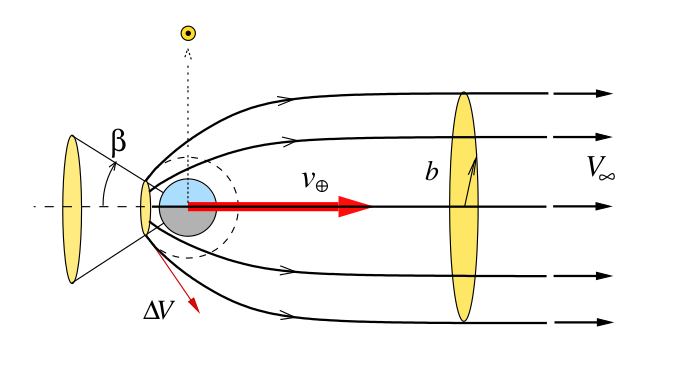
\includegraphics[scale=0.5]{./plots/hyperbola}
	\caption{Òrbita hiperbòlica de sortida de l'esfera d'influència del planeta.}
	\label{esquema_hyperbola}
\end{figure}
A la figura \ref{esquema_hyperbola} es veuen els elements rellevants que s'han d'obtenir.
\section{Velocitats a la sortida}
Per tal de determinar la hipèrbola de sortida, el primer pas és trobar les velocitats planetocèntrica i heliocèntrica de la sonda ,$V_{\infty}$ i $V_1$ respectivament, en el moment de sortida de l'EdI del planeta. La velocitat planetocèntrica, $V_{\infty}$, s'obté a partir de la velocitat heliocèntrica de la sonda, $V_1$, i de la velocitat heliocèntrica del planeta d'origen, $V_{P0}$, de la següent manera:
\begin{equation}
\vec{V}_{\infty} = \vec{V}_{1} - \vec{V}_{P0}
\end{equation}
Per tal d'obtenir tant $\vec{V}_{1}$ com $\vec{V}_{P0}$ de manera senzilla i genèrica, s'ha elaborat una funció de MATLAB, que a partir dels elements orbitals i de l'anomalia mitjana que tenia un cos en òrbita en un temps de referència, calcula la posició i la velocitat d'el cos en un instant determinat de temps. El codi d'aquesta es pot veure a la Secció \ref{OrbitalVectors}.

D'aquesta manera, s'utilitzen els elements orbitals del planeta d'origen en J2000 per a obtenir la seva posició i velocitat en l'instant $t_1$, i s'utilitzen els elements orbitals i l'anomalia mitjana de l'òrbita interplanetària, calculats en la secció anterior, fent servir com a temps de referència el propi instant $t_1$.

\section{Òrbita planetocèntrica hiperbòlica}
A les classes de l'assignatura s'ha arribat a les següents relacions \cite{Calaf2017d}:
\begin{equation}
a = \frac{\mu}{V_{\infty}^{2}}
\end{equation}
\begin{equation}
e = 1 + \Big(\frac{V_{\infty}}{V_{o}}\Big)^2
\end{equation}
\begin{equation}
\cos(\beta) = \frac{1}{e}
\end{equation}
\begin{equation}
b = a\sqrt{e^2-1}
\end{equation}
\begin{equation}
V_o = \sqrt{\frac{\mu}{r_o}}
\end{equation}
On:
\begin{itemize}
	\item a és el semieix major.
	\item e és l'excentricitat.
	\item $\beta$ és l'angle de l'asímptota. Veure fig.\ref{esquema_hyperbola}.
	\item b és el paràmetre de sortida. Veure fig.\ref{esquema_hyperbola}.
	\item $V_o$ és la velocitat que porta la sonda en l'òrbita d'aparcament de radi $r_o$.
	\item $\mu$ és el paràmetre de gravitació estàndard del planeta. (GM)
	\item $V_{\infty}$ representa el mòdul de la velocitat planetocèntrica que porta la sonda al sortir del planeta.
\end{itemize}
Aquests càlculs s'han portat a terme mitjançant el codi de la secció \ref{outHyperbola}.
\section{DeltaV}
Per trobar l'impuls que s'ha de subministrar s'aplica conservació d'energia cinètica:
\begin{equation*}
\frac{1}{2}V_{\infty}^2 =\frac{1}{2}(V_o + \Delta V)^2 - \frac{\mu}{r_o}
\end{equation*}
Arribant així a:
\begin{equation}
\Delta V = \sqrt{V_{\infty}^2+2V_{o}^2} - V_o
\end{equation}
